\documentclass[final,hyperref={pdfpagelabels=false}]{beamer}
\mode<presentation>{\usetheme{Lankton}}
\usepackage{times}
\usepackage{ragged2e} %% justify the text.
\usepackage{amsmath,amsthm, amssymb, latexsym}
\boldmath
\usepackage[english]{babel}
\usepackage[latin1]{inputenc}



\usepackage{ragged2e}

\usepackage{graphicx}
\graphicspath{{figures/}}
\usebackgroundtemplate%
{%
    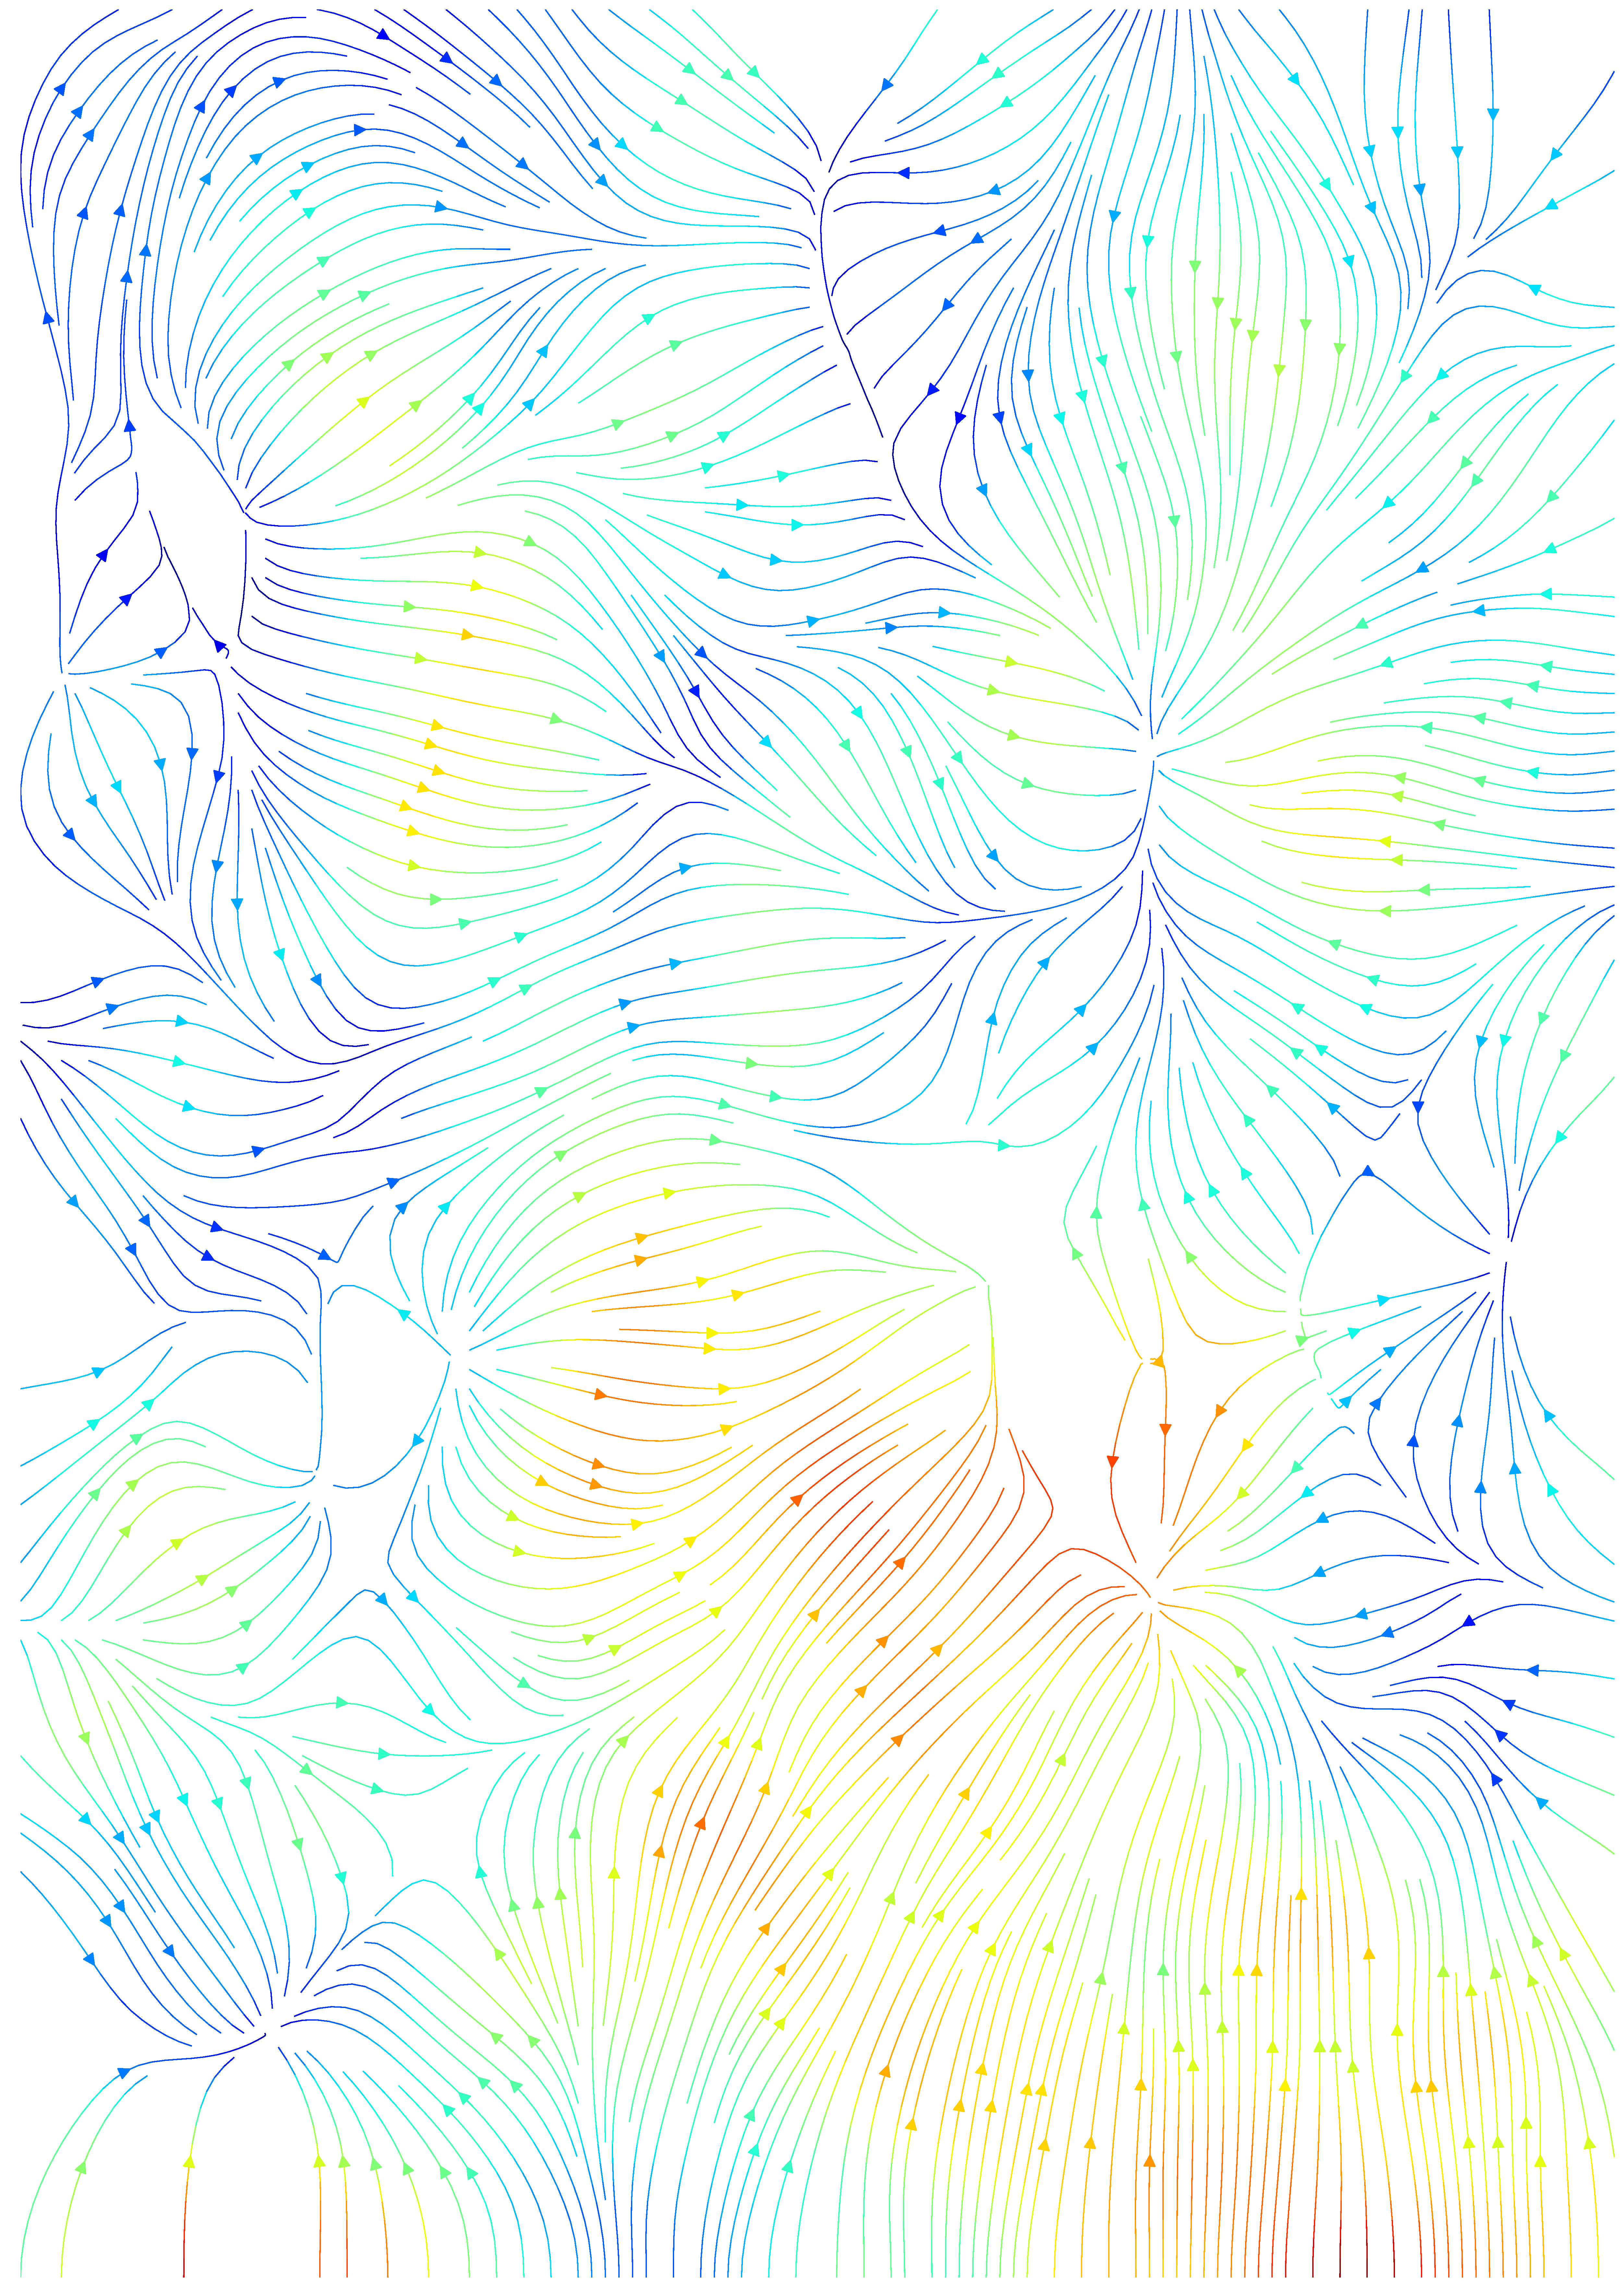
\includegraphics[width=\paperwidth,height=\paperheight]{electric_streams.pdf}%
}

\addtobeamertemplate{block begin}{\pgfsetfillopacity{0.5}}{\pgfsetfillopacity{1}}
\addtobeamertemplate{block alerted begin}{\pgfsetfillopacity{0.5}}{\pgfsetfillopacity{1}}
\addtobeamertemplate{block example begin}{\pgfsetfillopacity{0.5}}{\pgfsetfillopacity{1}}

% \usepackage[orientation=portrait,size=custom,width=40,height=80,scale=.6,debug]{beamerposter}
\usepackage[orientation=portrait,size=a0,scale=1]{beamerposter} %% this can scale the entire poster to make it smaller or bigger.

%-- Header and footer information ----------------------------------
\newcommand{\footleft}{Thunderstroms \& elementary particle acceleration, 2018}
\newcommand{\footright}{email: mihail.zelenyy@phystech.edu}
\title{Reactor like TGE model}
\author{Alexander Nozik \inst{1,2}, Mikhail Zelenyi  \inst{1,2,3}, Egor Stadnichuk \inst{1,2}}
\institute{Institute for Nuclear Research of RAS \and
    Moscow Institute of Physics and Technology (State University) \and
    Space Research Institute of RAS}
%-------------------------------------------------------------------


%-- Main Document --------------------------------------------------
\begin{document}
    
    \begin{frame}{}
        % 
        \begin{columns}[t]
            % 
            %     %-- Column 1 ---------------------------------------------------
            \begin{column}{0.32\linewidth}
                
                %-- Block 1-1
                \begin{block}{Introduction}  \justifying
                    Many previous works point to the fact that electric field inside the thundercloud is high enough to accelerate electrons and produce secondary electromagnetic showers ~\cite{gurevich1992runaway, gurevich1999lightning,dwyer2003fundamental,dwyer2011low}. The acceleration of electron is possible under two conditions:
                    \begin{itemize}
                        \item The strength of the field is higher than so-called critical field. The value of the field equals energy loss of minimally ionizing electron per length unit.
                        \item The initial electron energy is high enough to be close to minimally ionizing energy.
                    \end{itemize}
                    
                    But these model have next disadvantages:
                    \begin{itemize}
                        \item The major problem of all of these models is that that while field strength is higher than critical field, the multiplication coefficient for showers is rather small and can?t describe any observed effects.
                        \item   The crucial part of this work is additional account for escaping high energy gamma-rays in the acceleration process. Escaping photons with energy higher than 1 MeV could produce (via photo-effect or compton-effect) new electrons with energy high enough to start separate acceleration process. These electrons are produced not in vicinity of first accelerator, but separated by free path of gamma ray which could amount up to few km. Thus these secondary accelerators could not be accounted by any local model.
                        \item 
                    \end{itemize}
                    
                    Additionally, the field map calculation shows that field directions in two points of a thundercloud separated by distances more than 500 m are mostly uncorrelated, meaning that direction of new accelerator is more or less random relative to the initial accelerator.
                    If the size of a thundercloud is much larger than mean free path of gamma-ray, one can observe a chain reaction, where photons are produced in elementary accelerator cells with given local multiplication coefficient depending on local field strength and then create additional elementary accelerator cells in separate places. Some of photons could be absorbed without creating additional cell. For example it could happen in case local field direction is opposed to photon and therefore produced electron momentum. Accounting for such effects as well as loss of photons through borders of a thundercloud, one can get a global multiplicative coefficient. Obviously, in case global multiplication coefficient is larger than 1, one can observe an exponential rise in number of elementary accelerator cells and therefore total radiation level (gamma, infrared and neutron) and ionization. Also for coefficient slightly less than 1, one gets slow exponential decay of radiation background.
                    \begin{figure}[htb]
                        \centering
                        \includegraphics[width=1\columnwidth]{cell.pdf}
                        \caption{\textit{Cell} - cylinder with 100 meter radius and height }
                    \end{figure}
                    The described model is not unlike chain reaction process in nuclear reactor, so it could be called reactor-like terrestrial gamma enhancement model (RL-TGE).
                \end{block}
                
                %-- Block 1-2
                %      \begin{block}{}
                %
                %      \end{block}
                %
                %      %-- Block 1-3
                %      \begin{block}{Columns}
                %      \end{block}
                
            \end{column}%1
            
            %-- Column 2 ---------------------------------------------------
            \begin{column}{0.32\linewidth}
                
                %-- Block 2-1
                \begin{block}{Proof of concept}  \justifying
                    For fast checking the potential of our idea, we considered a simple model:  
                    \begin{itemize}
                        \item One variable -- the global coefficient of gamma multiplication,
                        \item Gamma multiplication occurs by Poisson distribution, momentum direction of generated gamma is defined by the electric field value,
                        \item Chaotic electric field: in every point of cloud, field has constant magnitudes and random direction by uniform distribution,
                        \item Energy of particle not taken into account, propagation of gamma based on exponential distribution with fixed free mean path,
                        \item Cloud size is equal 1 kilometer. 
                    \end{itemize}
                    This model is implemented as program on Kotlin programming language, which use next algorithm: in during one iteration program samples range of photons, propagations its, deletes photons which leave the cloud, samples field direction and number of new photons. Program stops when it reaches the limit of particles or all photons die.
                    As a result, we get the following evolution of the numbers of gammas for different coefficient of gamma multiplication:
                    \begin{figure}[htb]
                        \centering
                        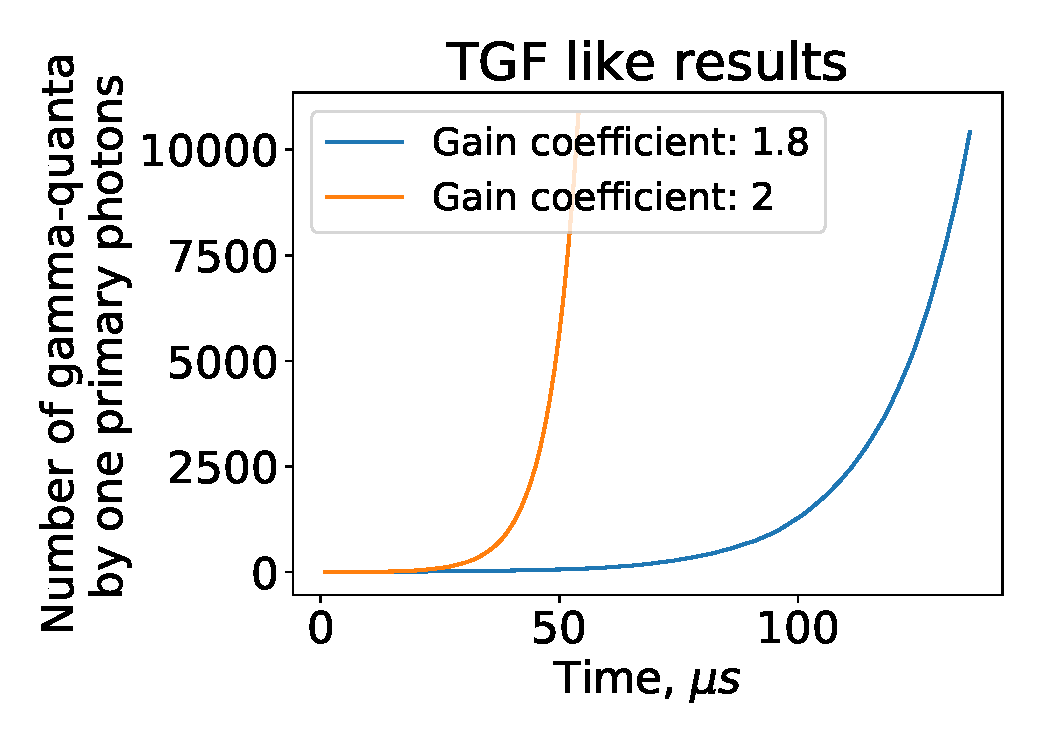
\includegraphics[width=1\columnwidth]{proofTGF.pdf}
                    \end{figure}
                    \begin{figure}[htb]
                        \centering
                        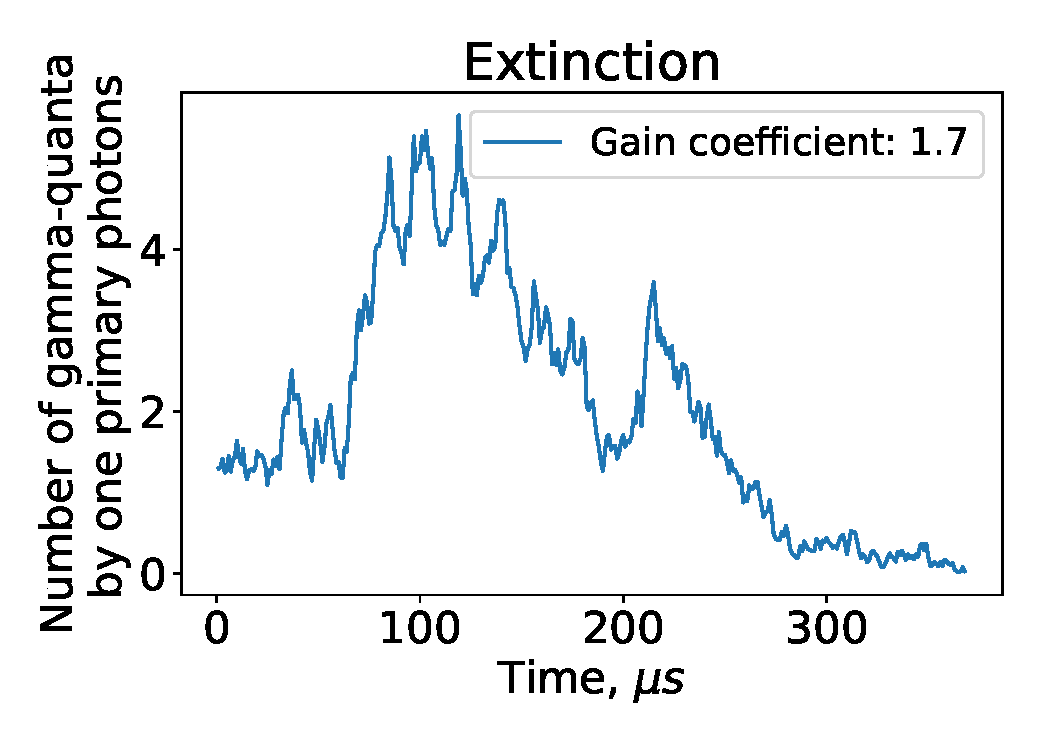
\includegraphics[width=1\columnwidth]{Extinction.pdf}
                    \end{figure}
                    \begin{figure}[htb]
                        \centering
                        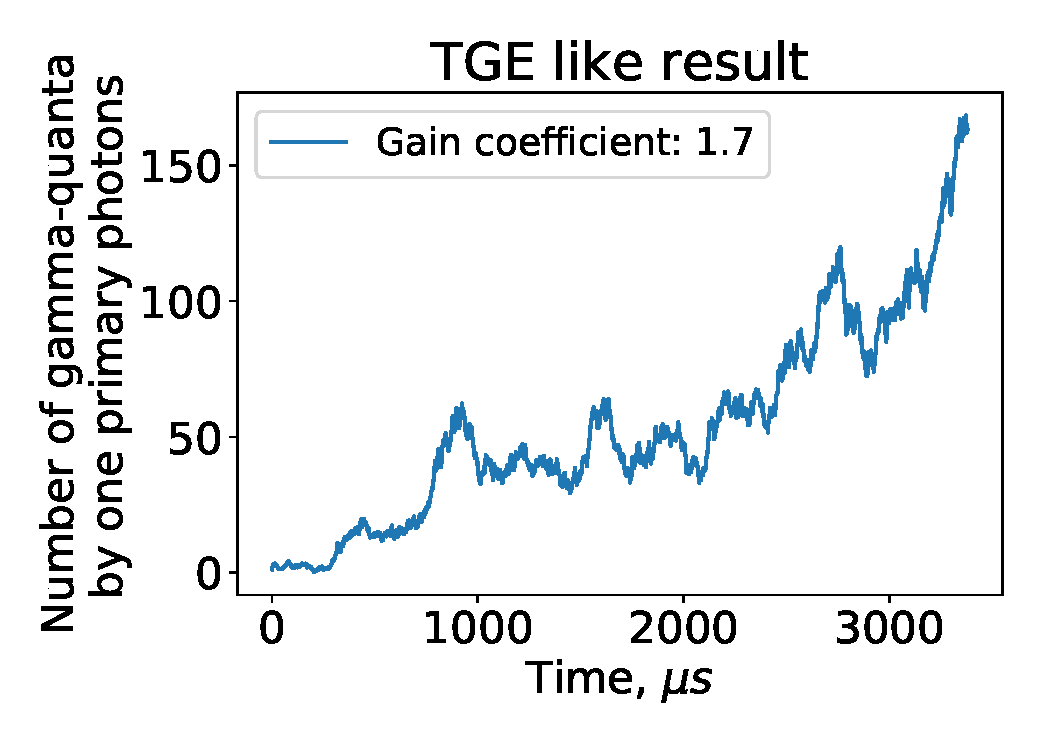
\includegraphics[width=1\columnwidth]{proofTGE.pdf}
                    \end{figure}
                \end{block}
                
                %-- Block 2-2
                \begin{block}{Some implications}  \justifying
                    \begin{itemize}
                        \item Long life time of Gamma-ray enhancement,
                        \item Slow increase of the air ionisation,
                        \item The angular distribution of gamma-rays depends on the main direction of electric field, but it is more isotropic then in Dwyer and Gurevich models,
                        \item TGF and TGE have identical nature and type of the event is defined by the state of the cloud.
                        
                    \end{itemize}
                \end{block}
                %
                %      %-- Block 2-3
                %      \begin{block}{Pictures}
                %
                %      \end{block}
                
            \end{column}%2
            
            %-- Column 3 ---------------------------------------------------
            \begin{column}{0.32\linewidth}
                
                %-- Block 3-1
                \begin{block}{Improved model}
                    Improved model clarify  rough approximations of simple model, namely:
                    \begin{itemize}
                        \item The map of the electric field is defined by fractal model ~\cite{Iudin:2018}
                        \item The photons range is computed exactly
                        \item The spectrum of secondary particle from cell is simulated by GEANT4~\cite{ALLISON2016186}
                        \item The calculation of energy spectrum of gamma-rays leaving cloud
                    \end{itemize}
                    
                    
                    
                    
                \end{block}
                
                %-- Block 3-2
                \begin{block}{Conclusion}
                    
                \end{block}
                %
                %-- Block 3-3
                \begin{block}{Literature}
                    \bibliographystyle{amsalpha}
                    \bibliography{references}{}
                \end{block}
                
            \end{column}%3
            
        \end{columns}
        
        %	\begin{block}{Conclusion} \justifying
        %Adaptive optics is a technique that allows to compensate the impact of atmospheric turbulence in real-time thus improving the quality of astronomical images. Design of the controller is the next stage of this research project.
        %	\end{block}%-- Block 1-2
        
    \end{frame}
\end{document}